\documentclass[conference,letterpaper]{IEEEtran}
\usepackage[T1]{fontenc}
\usepackage{amsmath,amssymb,booktabs,graphicx,microtype,xurl}
\usepackage[hidelinks]{hyperref}
\setlength{\emergencystretch}{2em}
\newcommand{\FWwiAttr}{0.7688}
\newcommand{\FWwiGraph}{0.7888}
\newcommand{\FWwiAug}{0.7626}
\newcommand{\FOlistAttr}{0.6919}
\newcommand{\FOlistGraph}{0.7842}
\newcommand{\FOlistAug}{0.7414}
\newcommand{\FDataCoAttr}{0.6962}
\newcommand{\FDataCoGraph}{0.6750}
\newcommand{\FDataCoAug}{0.6962}
\newcommand{\FBpiAttr}{0.1242}
\newcommand{\FBpiGraph}{0.5734}
\newcommand{\FBpiAug}{0.1492}
\newcommand{\WdcAttr}{0.5369}
\newcommand{\WdcAug}{0.5584}
\newcommand{\WdcEmb}{0.3919}

\title{Traceable Entity Reconciliation with Gated Transaction Context: A Five-Dataset Evaluation}
\author{\IEEEauthorblockN{Anonymous research draft}}
\begin{document}
\maketitle
\begin{abstract}
Entity reconciliation changes both integrated identities and downstream query answers. We evaluate an auditable prototype that preserves typed source observations and lineage, combines attributes with gated transaction context, and adds one-to-one canonical links. Five evaluations cover fidelity, matching, queries, robustness/calibration and scaling across WWI, Olist, DataCo, BPI Challenge 2019 and all 27 official WDC Products pairwise configurations. On common ambiguous candidates, three-seed mean F1 changes from \FWwiAttr{} to \FWwiGraph{} on WWI, \FOlistAttr{} to \FOlistGraph{} on Olist, \FDataCoAttr{} to \FDataCoGraph{} on DataCo, and \FBpiAttr{} to \FBpiGraph{} on BPI, whose baseline is coarse history descriptors. Flat SQL and graph context produce equal scores, isolating evidence from representation. WDC has no transaction graph; adding a frozen embedding cosine raises fully unseen mean F1 from \WdcAttr{} to \WdcAug{}. Eighteen official WDC configurations have development-test offer overlap. Query controls maintain SQL/graph parity but reveal identity-dependent errors. Forty-five scaling trials complete while candidate recall deteriorates under bounded retrieval and replication. The exploratory evidence supports traceable integration and conditional contextual benefit, not universal gains, graph-specific predictive superiority or production scalability. No human study was performed.
\end{abstract}
\begin{IEEEkeywords}
entity resolution, knowledge graphs, transaction context, provenance, reproducible evaluation
\end{IEEEkeywords}

\section{Introduction}
Reconciling records across purchasing, warehouse, finance and customer systems is a consequential data-management task. A missed identity omits valid cross-source paths. A false merge attributes transactions to the wrong entity and can distort answers even when query execution is internally consistent. Descriptive attributes provide an initial signal, while histories offer categories, activities, dates and compatible numerical observations. Histories can also be sparse or misleading. A graph representation alone does not establish that those observations improve matching.

We present a prototype connecting typed ingestion, provenance, attribute/context matching, constrained canonical views and independent query controls. Source records remain intact. Truth and original entity keys are excluded from scoring; canonical links are added after decisions. Our contribution is this evaluated artifact and its controls: native SQL reference sets for ingestion, common candidates and tuning catalogs for matching, relational/graph evidence parity, oracle-based query accuracy, frozen perturbations, and scaling with full positive-pair denominators. The evidence includes negative results rather than assuming context always helps.

Five questions guide the study. RQ1 asks whether ingestion preserves source relationships and lineage. RQ2 asks whether gated context improves matching over attributes on identical candidates. RQ3 separates downstream identity accuracy from SQL/graph answer equality. RQ4 examines defects, ablations and calibration. RQ5 measures computational and retrieval trade-offs at increasing projected workload sizes. Corresponding experiments E1--E5 cover all applicable datasets. WDC has no ERP transaction graph and therefore no E3 ERP query workload. A human study was excluded.

WWI and WDC were the original primary datasets; Olist, DataCo and BPI expand task diversity. The expanded run is exploratory. In particular, an Olist source adapter was adjusted after a context-availability diagnostic on test records, before fitting its expanded models. All amendments and earlier results are retained. Freezing later models/policies does not make the adapter design preregistered.

\section{Related Work and Position}
Collective entity resolution already uses relational evidence between references~\cite{collective}. GraphER combines dependency knowledge and graph neural processing~\cite{grapher}. We do not claim to introduce relational matching or reproduce those systems: explicit context summaries and evidence parity controls are our evaluated mechanism.

Ditto fine-tunes pretrained language models for pair classification~\cite{ditto}. Sentence-BERT supplies similarity representations~\cite{sbert}; MiniLM investigates transformer distillation~\cite{minilm}. Our executable neural reference is a frozen, quantized all-MiniLM-L6-v2 encoder~\cite{modelcard}, supplying one cosine feature to the same learner catalog as lexical attributes. It is not a reproduced Ditto baseline or a fine-tuned transformer comparison.

Blocking and filtering constrain search and recall~\cite{blocking}; we therefore report candidate-conditioned and full-pipeline accuracy separately. WDC Products supplies hardness, development-size and unseen-product dimensions~\cite{wdc}, all retained here with split-overlap audits. LIS illustrates industrial knowledge-graph integration~\cite{lis}, but our public-source prototype does not establish industrial adoption. PROV-O motivates lineage concerns~\cite{prov}; our property lineage is not a complete RDF conformance claim. An artifact-building design-science perspective~\cite{designscience} supports explicit requirements and technical evaluation, while calibration is assessed separately from ranking~\cite{calibration}.

\section{Method and Design Controls}
\subsection{Identity, evidence and representation}
\begin{figure*}[t]\centering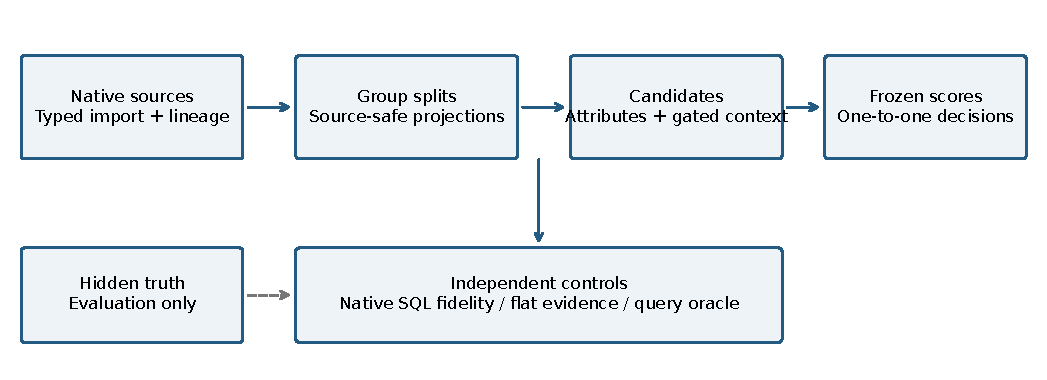
\includegraphics[width=\textwidth]{figures/architecture.pdf}
\caption{Source-preserving pipeline with separate evaluator controls. Canonical links are added after scoring; hidden truth is not a matching input.}\label{fig:architecture}\end{figure*}
Let $R_A,R_B$ be independently named source-view records with type $t(r)$ and local identifier $u(r)$. Evaluator-only original identity $z(r)$ defines $y_{ab}=\mathbb{1}[z(a)=z(b)]$ for same-type cross-source pairs. Matching excludes $z$, original master keys and canonical identifiers. Local UIDs address nodes and deterministic ties but do not enter text features. Native data are imported into a typed property graph with declared mappings and lineage. Matching projections expose local masters, transactions and observed category/activity paths; full native import and matching population are different scopes.

The design requires traceability, type awareness, conservative context use, exclusion of circular evidence, comparable controls and reproducibility. Expanded native source graphs are SQLite-backed; matching projections and original WWI use NetworkX. This is a local prototype, not a distributed graph/relational database comparison. Native SQL foreign-key joins provide E1 reference relationships. A separate flat SQL extractor joins the permitted matching projection to test context parity with graph traversal.

Lineage completeness is the fraction of source-table, batch and mapper fields present. Summary contributions use the smaller completeness value of a master and its transaction. WWI native anchors additionally use visible attribute completeness. These weights quantify metadata availability, not empirically estimated correctness. Misleading edges can retain complete lineage.

\subsection{Attributes, context and score gating}
Attributes contain 20 features covering character/token similarities, training-only character TF-IDF cosine, category/brand agreement, description similarity, price/currency compatibility, missingness, numeric/alphanumeric tokens, explicit sizes and length. WWI exposes QuantityPerOuter through three further features to every learned attribute comparator. Attribute currency equality treats two empty strings as equal; no currency conversion or known-currency guarantee is implied. Common learners use scikit-learn~\cite{sklearn}.

The pinned MiniLM encoder uses quantized CPU ONNX inference, batch 64, 256 tokens, mean pooling and L2 normalization. Allowed name/brand/description text is truncated to 2,000 characters first. IDs, truth and prices are excluded. A 384-dimensional record embedding yields a single pair cosine; augmented attributes concatenate that scalar, and embedding-only learning uses it alone. No encoder fine-tuning is performed.

Generic context has 16 dimensions: category/activity cosine, degree similarity, distinct shared tags, weighted support, date mean/span, quantity mean/deviation, amount mean/deviation, availability/unit flags, category contradiction and context availability. Numerical comparisons use declared units. The generic gate requires at least two distinct projected category tags and support weight at least one. Prefix-only missing-category markers can count, so this is not a guarantee of two informative categories or independently resolved entities.

WWI combines five native master dimensions, 15 transaction dimensions and the preserved independent-anchor gate. Unique exact normalized same-type names and compatible categories infer anchors, excluding candidate endpoints. Stock-supplier and co-supplied-stock paths provide support; at least two distinct anchors and weighted support one are required. QuantityPerOuter is not anchor evidence. It converts purchased stock-item outers to stock units; supplier outers, signed stock movements and absent finance quantities remain distinct.

For calibrated attribute probability $p_A$, contextual probability $p_C$ and support $h$, the graph score is
\begin{equation}
 p_G=h p_C+(1-h)p_A.
\end{equation}
Unsupported scores equal attribute scores, but acceptance may differ because each method can have its own policy threshold. Support does not guarantee correctness. If flat and graph extraction yield equal features/support, a common estimator, calibrator and policy must produce equal scores. Thus predictive benefit is attributable to permitted evidence, not storage representation.

\subsection{Candidates, fitting and decisions}
E2 WWI preserves its original token-prefix/category block under a two-million-pair guard, without a per-left K cap. Other graph tasks use bounded K=32 common candidates. A pair is ambiguous when character similarity is below 0.95 or its left record has more than one token-sort-similar candidate (similarity at least 0.65). Every method uses that same diagnostic stratum.

Original canonical groups are split before aliases; generic train/validation/test proportions are 60/20/20 and WWI retains its original split. Validation groups are partitioned into selection, calibration and policy roles; cross-role pairs are omitted. Each learned family compares five estimators: class-balanced standardized logistic regression with C=0.1,1,10 and class-balanced 160-tree random forests with depths 8/16 and minimum leaf two. Selection uses weighted F1 with its own threshold; catalog order breaks ties. The chosen estimator is sigmoid-calibrated on a separate role by logistic regression on clipped probability logits. A third role selects acceptance by weighted F1, preferring higher thresholds on ties. Role weights restore full-validation candidate prevalence, not test prevalence. Rejection is bounded by 0.10 and acceptance. Models and policies are saved before test-label metrics.

For E5 bounded retrieval, validation chooses K from 8/16/32 with recall target 0.95, posting cap 8K, maximum 12 keys and two-million output guard. WWI chooses K=8; other graph tasks choose K=32 without reaching the target. Posting hashes and visible name similarity determine retrieval order. The emitted-pair bound does not bound every internal ranking operation.

Greedy descending-score acceptance enforces type consistency and one-to-one endpoint use. Accepted source records point to added canonical entities; rejected, abstained and conflicting candidates remain auditable. This handles the evaluated two-source problem, not general transitive many-duplicate clustering.

\subsection{Comparators and adapter-specific ablations}
B0 exact requires normalized name/category agreement and nonmissing name; B1 uses token-sort similarity. B2 learns attributes, B3 the embedding cosine and the augmented reference both. B5 uses gated graph context; B4 uses independently extracted SQL context and the same model/policy. NoContext shares B2's score/threshold. NoGate uses the weighted learner without fallback, with a separately selected policy, not a separately trained gate-free model. NoSupport trains without explicit support features but retains the original final gate.

Generic OneHop removes category traversal and uses local activity/numerical support; WWI also transforms its native typed master neighborhood. NoTransactions removes WWI's entire 15-dimensional transaction block, whereas generic adapters remove date/numerical/unit features but retain category/activity/degree. UnitWeights changes inputs to the frozen weighted estimator/policy; it is not a retrained ablation. These distinctions limit cross-adapter interpretation.

\section{Datasets and Experimental Protocol}
\begin{table*}[t]\centering\small\begin{tabular}{lrrrl}
\toprule
Dataset & Native nodes & Native edges & Groups & Train / val. / test \\
\midrule
WWI & 249,786 & 274,856 & 240 & 143 / 48 / 49 \\
Olist & 1,569,937 & 1,775,243 & 2,913 & 1747 / 583 / 583 \\
DataCo & 267,103 & 607,478 & 1,500 & 900 / 300 / 300 \\
BPI2019 & 1,926,659 & 7,138,894 & 1,378 & 826 / 276 / 276 \\
\bottomrule
\end{tabular}

\caption{Full-source graphs versus matching groups and fixed splits. Each matching group supplies two source views; graph-node totals are not training-record totals.}\label{tab:profiles}\end{table*}
\subsection{Source scope and truth}
WWI is Microsoft's fictional OLTP sample~\cite{wwi}. Six in-scope native tables yield 249,786 nodes/274,856 edges. Matching has 13 suppliers/227 stocks in purchasing and warehouse/finance views, including the preserved first 5,000 sorted movement rows; E1 covers the complete in-scope movement source. The fixed 49-group test has only three suppliers. Seeds vary aliases, not independent populations.

Olist imports all nine official version-2 CSVs and postal-prefix grouping nodes~\cite{olist}. All 2,913 eligible natural repeat-customer groups have two distinct observed accounts with item histories; customer\_unique\_id is evaluator-only. Visible attributes are city/state/postal prefix, without customer names. Up to 40 order items per view provide price, item-row count and declared order/product/seller joins. Amounts are unspecified source units, not paid spend. Seller-state context was added before fitting after a test-context support diagnostic, making this adaptation exploratory.

DataCo uses only the version-5 structured CSV (180,519 rows/53 columns), rather than its clickstream files~\cite{dataco}. Publisher acquisition returned 403; a documented mirror supplies the checked CSV, without publisher-byte equivalence. From 10,075 eligible customers, stable pre-alias hashing selects 1,500, with disjoint orders and controlled name defects. Email/password fields are excluded from graph/model attributes. These are controlled aliases, not independently labelled natural dirty identities.

BPI imports all 251,734 cases/1,595,923 events, checking publisher MD5 and eight relation sets~\cite{bpi}. All 1,378 eligible vendors supply disjoint case histories. Vendor names/IDs and company/source identifiers are excluded from matching text. Baseline name/category/brand fields are separately derived modal spend-area/document-type/classification descriptors. BPI therefore tests detailed history beyond coarse history, not literal supplier attributes. Quantity is absent; amount is first-event anonymized cumulative case value, not summed cumulative events or payments.

WDC retains all official pairwise configurations~\cite{wdc,wdcsite}. Used files contain 155,957 pair observations, 10,422 offers and 1,600 groups, distinct from whole-benchmark counts. Each official test has 4,500 pairs/500 positives. Nine hardness/size settings times three seeds yield 27 fitted bundles reused over three unseen variants: 81 evaluations, not 81 independent fits. Eighteen cells have training-test and/or validation-test offer overlap. We flag them and save offer-disjoint subset metrics without changing official pairs. Fully unseen cells have zero offer overlap; sizes reuse test pools.

\subsection{Five linked evaluations}
E1 checks complete in-scope counts, native SQL relation equality, lineage, dangling edges and idempotence. WDC checks offers, pair schema/counts and split hashes. E2 has 12 graph seed runs with 13 methods and 81 WDC cells with five methods. Blocking recall is retained positives divided by the complete cross-source true-pair set $T$. End-to-end pair F1 is $2TP/(TP+FP+|T|)$, before one-to-one constraints. Accepted false merges are audited separately.

Paired per-seed intervals use 1,000 canonical-group resamples on ambiguous candidates. With sampled group counts $m_g$, same-group pair weight is $m_g$ and distinct-group pair weight $m_gm_h$, shared by both classifiers. We report percentile endpoints without pooling seed populations, confirmatory testing or multiplicity-adjusted significance claims.

E3 executes eight adapted templates under unreconciled, predicted and oracle identities, normalizing answer tuples by source UID. Q2 local positive transactions and Q4 local typed paths are source-local controls; Q1 shared categories, Q3 amount/count attribution, Q5 positive transaction links, Q6 identities, Q7 tag-grouped totals and Q8 lineage depend on identity. SQL and graph answers are compared exactly under each map and with oracle truth. Monetary aggregation is cent-rounded source units; overlapping tag classes in Q7 do not form a global spend rollup. The four adapted task sets are not 32 independent workloads. WWI additionally retains native Q1--Q8, including purchasing/finance lineage semantics.

E4 freezes candidates, models and policies across clean/no-support conditions, attribute noise 30/50\%, optional missingness 10/30/50\%, edge removal 15/30\%, typed misleading rewiring 15/30\% and provenance missingness 30\%. WDC has six attribute-only conditions. These are controlled defects, not production prevalence estimates. Frozen pairs omit effects of corruption on retrieval. Raw/calibrated Brier, log loss and ten equal-width-bin ECE are saved with reliability and preconstraint coverage/risk.

E5 measures 1k/10k/100k projected graph nodes or offers, three trials each. Complete graph units can overshoot targets; later growth replicates original groups. All cross-replica true pairs remain in recall denominators, without copy-suffix features. Query timing uses common per-copy oracle identities, one warmup and five measured executions, with graph/SQL preparation separately timed. RSS is sampled every 50 ms. Supplemental isolated scorer/canonicalization costs are distinct from main pipeline timing.

\section{Results}
\subsection{E1: fidelity}
All four in-scope native graph imports have exact reference relation sets, full lineage, no dangling edges and idempotent edge import. Olist checks ten relations, DataCo six, BPI eight and WWI eight FK controls. WDC verifies schema/counts, offer identities, evaluator-label exclusion and source split hashes. These are preservation checks for declared mappings, not proof of source correctness or completeness of every business interpretation.

\subsection{E2: matching and accepted identities}
\begin{table*}[t]\centering\small\begin{tabular}{lrrrr}
\toprule
Method & WWI & Olist & DataCo & BPI \\
\midrule
Exact & 0.3402 & 0.7502 & 0.1994 & 0.0538 \\
Fuzzy & 0.7145 & 0.1039 & 0.2001 & 0.0639 \\
Attributes & 0.7688 & 0.6919 & 0.6962 & 0.1242 \\
Embedding & 0.4157 & 0.2327 & 0.2594 & 0.0840 \\
Attributes + embedding & 0.7626 & 0.7414 & 0.6962 & 0.1492 \\
Flat SQL context & 0.7888 & 0.7842 & 0.6750 & 0.5734 \\
Gated graph context & 0.7888 & 0.7842 & 0.6750 & 0.5734 \\
No context & 0.7688 & 0.6919 & 0.6962 & 0.1242 \\
No gate & 0.7763 & 0.7806 & 0.6710 & 0.5734 \\
No support features & 0.7879 & 0.7913 & 0.6780 & 0.5465 \\
No transaction summaries & 0.7887 & 0.7474 & 0.6790 & 0.4264 \\
One hop & 0.7688 & 0.6919 & 0.6946 & 0.4827 \\
Unit-weight inputs & 0.7440 & 0.7842 & 0.6750 & 0.5734 \\
\bottomrule
\end{tabular}

\caption{Three-seed mean conditional F1 on common ambiguous candidates. Adapter-specific NoTransactions/OneHop semantics and frozen UnitWeights are described in Section III.}\label{tab:match}\end{table*}
Graph-minus-attribute ambiguous mean F1 is +0.0200 on WWI, +0.0923 on Olist, -0.0212 on DataCo and +0.4492 on BPI (Table~\ref{tab:match}). DataCo refutes universal improvement. Olist exact F1=0.7502 exceeds learned attributes=0.6919, so the learned comparator is not best across all controls. BPI's large effect is conditional on its coarse modal baseline and cannot imply the same gain for supplier-name matching.

\begin{figure*}[t]\centering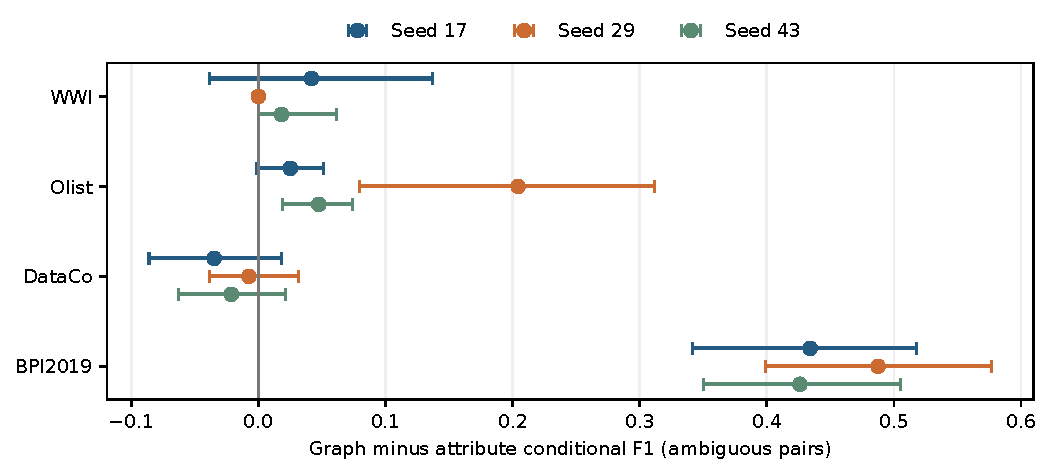
\includegraphics[width=.88\textwidth]{figures/context_effects.pdf}
\caption{Per-seed ambiguous F1 effects with paired endpoint-multiplicity bootstrap percentile intervals. Alias seeds share source populations; no pooled confidence claim is made.}\label{fig:effects}\end{figure*}
WWI's seed-29 contrast is zero; the other seeds have small gains. Olist effects vary substantially and seed 17 crosses zero. DataCo effects are negative with intervals crossing zero. BPI's three intervals are above zero under the adapted task (Fig.~\ref{fig:effects}). Small WWI groups and exploratory construction constrain statistical interpretation.

\begin{table*}[t]\centering\small\begin{tabular}{lrrrrr}
\toprule
Dataset & Groups & Candidates & Block R & Attr. F1 & Graph F1 \\
\midrule
WWI & 49 & 1314--1411 & 1.000 & 0.797 & 0.826 \\
Olist & 583 & 8815--8816 & 0.821 & 0.654 & 0.725 \\
DataCo & 300 & 8857--9016 & 0.874 & 0.674 & 0.649 \\
BPI2019 & 276 & 7850--8049 & 0.755 & 0.110 & 0.490 \\
\bottomrule
\end{tabular}

\caption{All-candidate end-to-end F1 before one-to-one decisions, with complete true-pair denominator. This differs from Table~\ref{tab:match}'s ambiguous conditional metric.}\label{tab:end}\end{table*}
Mean blocking recall is 1.000/0.821/0.874/0.755 for WWI/Olist/DataCo/BPI. End-to-end graph F1 becomes 0.826/0.725/0.649/0.490 (Table~\ref{tab:end}), revealing retrieval losses. Flat and graph scores agree within $10^{-12}$, making B4/B5 results identical. This identifies additional evidence rather than graph storage as the matching contribution. Clean generic lineage weights are one, so identical unit-weight results there cannot establish weighting benefit.

After one-to-one constraints, graph-method accepted links/false merges summed over three seed trials are 107/1 for WWI, 1,092/37 for Olist, 636/62 for DataCo and 372/54 for BPI. These trial counts reuse original entities. Persistent errors constrain claims about safe canonicalization; preconstraint stress false positives use a different denominator.

\subsection{WDC results and split audit}
Fully unseen mean F1 is 0.0000 exact, 0.3477 fuzzy, \WdcAttr{} attributes, \WdcEmb{} embedding-only and \WdcAug{} augmented attributes. The cosine feature adds 0.0215 mean F1, whereas embedding-only is weaker. This is a descriptive mean over nine correlated hardness/size cells and three seeds, without pooled interval or test-based unseen-variant selection.
\begin{table*}[t]\centering\small\setlength{\tabcolsep}{5pt}\begin{tabular}{rlrrrrrr}
\toprule
Hard & Size & Unseen & Attr. & Emb. & Attr.+emb. & Train $\cap$ test & Val. $\cap$ test \\
\midrule
20 & small & 0 & 0.529 & 0.357 & 0.570 & 0 & 4 \\
20 & small & 50 & 0.570 & 0.388 & 0.611 & 97 & 105 \\
20 & small & 100 & 0.570 & 0.390 & 0.600 & 0 & 0 \\
20 & medium & 0 & 0.587 & 0.389 & 0.583 & 0 & 4 \\
20 & medium & 50 & 0.603 & 0.411 & 0.620 & 155 & 105 \\
20 & medium & 100 & 0.587 & 0.416 & 0.613 & 0 & 0 \\
20 & large & 0 & 0.568 & 0.389 & 0.581 & 0 & 4 \\
20 & large & 50 & 0.605 & 0.414 & 0.627 & 269 & 105 \\
20 & large & 100 & 0.590 & 0.429 & 0.596 & 0 & 0 \\
50 & small & 0 & 0.533 & 0.342 & 0.543 & 0 & 4 \\
50 & small & 50 & 0.539 & 0.347 & 0.542 & 110 & 106 \\
50 & small & 100 & 0.535 & 0.370 & 0.548 & 0 & 0 \\
50 & medium & 0 & 0.555 & 0.381 & 0.564 & 0 & 4 \\
50 & medium & 50 & 0.567 & 0.377 & 0.571 & 162 & 106 \\
50 & medium & 100 & 0.538 & 0.417 & 0.555 & 0 & 0 \\
50 & large & 0 & 0.558 & 0.381 & 0.572 & 0 & 4 \\
50 & large & 50 & 0.588 & 0.377 & 0.607 & 274 & 106 \\
50 & large & 100 & 0.538 & 0.417 & 0.578 & 0 & 0 \\
80 & small & 0 & 0.446 & 0.323 & 0.450 & 0 & 4 \\
80 & small & 50 & 0.490 & 0.336 & 0.490 & 110 & 103 \\
80 & small & 100 & 0.470 & 0.347 & 0.482 & 0 & 0 \\
80 & medium & 0 & 0.467 & 0.329 & 0.471 & 0 & 4 \\
80 & medium & 50 & 0.519 & 0.369 & 0.529 & 159 & 103 \\
80 & medium & 100 & 0.498 & 0.385 & 0.524 & 0 & 0 \\
80 & large & 0 & 0.469 & 0.299 & 0.476 & 0 & 4 \\
80 & large & 50 & 0.531 & 0.371 & 0.529 & 272 & 103 \\
80 & large & 100 & 0.506 & 0.355 & 0.529 & 0 & 0 \\
\bottomrule
\end{tabular}

\caption{Every official WDC pairwise cell: hardness/unseen percentages; three-seed F1 means; distinct training-test and validation-test offer overlaps. Nonzero intersections flag contaminated official cells. Disjoint-subset metrics are separate diagnostics.}\label{tab:wdc}\end{table*}
Table~\ref{tab:wdc} reports both overlap types for all cells. Checking training-test overlap alone misses small seen cells that intersect validation. All official pairs are retained, but the 18 overlapping cells are not clean held-out evidence. Fully unseen and explicitly denominator-preserving disjoint subsets provide the cleaner diagnostics. No ERP context gain is inferred from WDC.

\subsection{E3: query consequences}
\begin{table}[t]\centering\footnotesize\begin{tabular}{lrrrr}
\toprule
Query & WWI & Olist & DataCo & BPI \\
\midrule
Q1 & 0.800 & 0.794 & 0.739 & 0.561 \\
Q2 & 1.000 & 1.000 & 1.000 & 1.000 \\
Q3 & 0.845 & 0.743 & 0.747 & 0.528 \\
Q4 & 1.000 & 1.000 & 1.000 & 1.000 \\
Q5 & 0.998 & 0.729 & 0.742 & 0.603 \\
Q6 & 0.832 & 0.743 & 0.747 & 0.528 \\
Q7 & 0.816 & 0.741 & 0.745 & 0.560 \\
Q8 & 0.931 & 0.729 & 0.742 & 0.594 \\
\bottomrule
\end{tabular}

\caption{Mean predicted-identity answer-set F1. Q2/Q4 are local controls; all oracle results are nonempty. SQL/graph answers agree under every identity control.}\label{tab:queries}\end{table}
All 288 adapted query rows satisfy SQL/graph equality; oracle accuracy is one. Q2/Q4 remain exact. Identity-sensitive queries recover otherwise absent paths while retaining task-specific errors (Table~\ref{tab:queries}). Olist Q6 is 0.743 and BPI Q6 0.528; BPI transaction-link Q5 is 0.603, demonstrating different downstream weighting of link errors. The 72 native WWI rows are recorded separately. Execution parity cannot certify an incorrect identity map, and no query macro-average conflates different source semantics.

\subsection{E4: robustness and calibration}
\begin{figure*}[t]\centering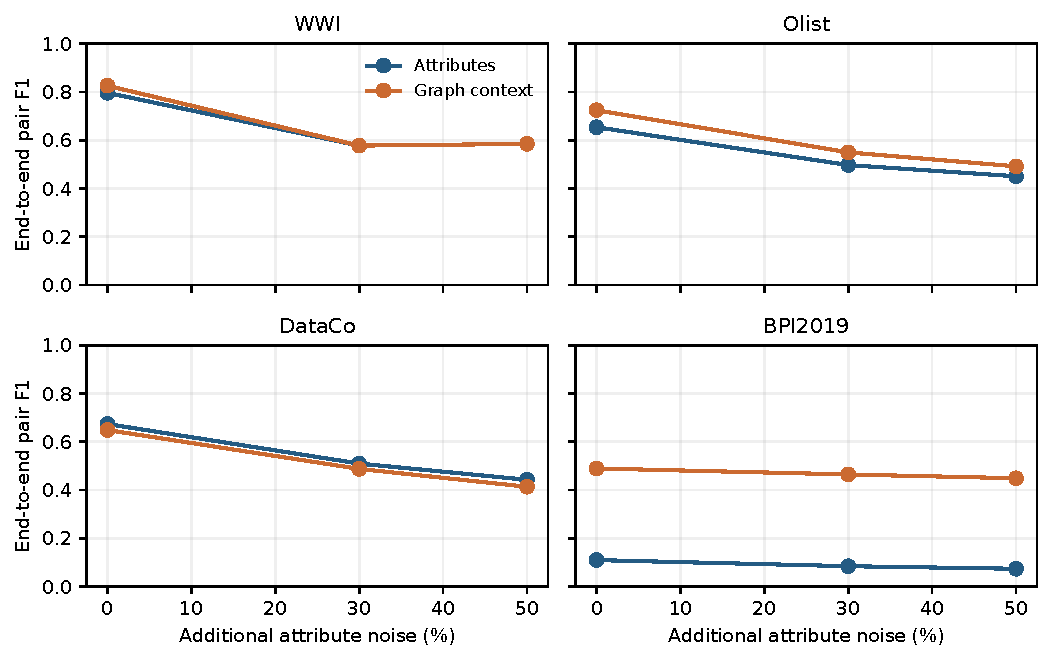
\includegraphics[width=.83\textwidth]{figures/attribute_stress.pdf}
\caption{Frozen-pair attribute stress: three-seed mean end-to-end F1. Retrieval is held fixed and controlled defect rates are not production prevalence estimates.}\label{fig:stress}\end{figure*}
The expanded study saves 1,872 graph robustness rows and 2,430 WDC rows. Complete scenario tables, reliability bins, coverage/risk and support subgroups accompany the technical supplement. Context can supply evidence after attribute corruption, but missing or misleading histories undermine that evidence. Metadata completeness cannot detect every wrong relation, and generic missingness tags can artificially satisfy support.

Clean ablations reject universal component benefits. BPI NoTransactions F1=0.4264 versus graph=0.5734, with categorical/activity context retained. WWI removes its whole transaction block yet changes from 0.7888 to 0.7887, limiting claims about that block's contribution. NoGate lowers WWI to 0.7763 but leaves BPI unchanged. NoSupport can exceed the full model on Olist/DataCo.

Calibration lowers mean raw losses/ECE in the reported attribute/graph candidate sets, but calibrated method comparisons remain mixed. DataCo Brier is 0.0129 attributes versus 0.0138 graph; Olist graph Brier/log loss are lower but ECE is 0.0182 versus attribute 0.0111. Candidate imbalance, small development roles and deployment-prior uncertainty prevent calibrated probability or threshold guarantees. Pair coverage/risk is preconstraint; final false merges are separately audited.

\subsection{E5: scale, retrieval and query timing}
\begin{table*}[t]\centering\small\setlength{\tabcolsep}{5pt}\begin{tabular}{lrrrrrrr}
\toprule
Dataset & Target & Actual & Match rec. & Pairs & Block R & Seconds & RSS GiB \\
\midrule
WWI & 1k & 1,021 & 36 & 132 & 1.000 & 0.25 & 0.32 \\
WWI & 10k & 10,722 & 96 & 356 & 1.000 & 1.87 & 0.37 \\
WWI & 100k & 100,729 & 974 & 3,896 & 0.705 & 24.46 & 0.70 \\
Olist & 1k & 1,000 & 414 & 2,309 & 0.966 & 0.57 & 0.32 \\
Olist & 10k & 10,001 & 4,308 & 47,913 & 0.722 & 7.56 & 0.48 \\
Olist & 100k & 100,001 & 43,176 & 687,264 & 0.397 & 109.13 & 2.91 \\
DataCo & 1k & 1,011 & 112 & 1,312 & 0.946 & 0.71 & 0.66 \\
DataCo & 10k & 10,001 & 1,150 & 17,074 & 0.820 & 6.58 & 0.70 \\
DataCo & 100k & 100,012 & 11,470 & 179,974 & 0.594 & 69.57 & 1.49 \\
BPI2019 & 1k & 1,032 & 50 & 270 & 0.920 & 0.50 & 1.08 \\
BPI2019 & 10k & 10,023 & 560 & 8,231 & 0.767 & 4.50 & 1.11 \\
BPI2019 & 100k & 100,014 & 5,566 & 88,716 & 0.172 & 47.62 & 1.49 \\
WDC & 1k & 1,000 & 1,000 & 12,638 & 0.990 & 0.96 & 2.00 \\
WDC & 10k & 10,000 & 10,000 & 160,137 & 0.837 & 18.74 & 2.11 \\
WDC & 100k & 100,000 & 100,000 & 1,606,844 & 0.336 & 373.05 & 3.27 \\
\bottomrule
\end{tabular}

\caption{All 15 workload points, medians of three main trials. Graph Actual counts projected nodes, WDC offers; Match rec. counts matching observations. Seconds are main pipeline timings; RSS is absolute process peak. Replicas enter full positive-pair denominators.}\label{tab:scale}\end{table*}
All 45 main trials complete. Largest-target median times are 24.46/109.13/69.57/47.62/373.05 s for WWI/Olist/DataCo/BPI/WDC; WDC absolute peak is 3.27 GiB (Table~\ref{tab:scale}). These projected workloads differ from million-node native E1 graphs and from 100,000 independently sourced masters. Largest-target blocking recall falls to 0.705/0.397/0.594/0.172/0.336. Finishing under a cap therefore does not establish recall-preserving scalability, and three-point capped-output slopes do not prove subquadratic computation.

At 100k projected graph nodes, warmed eight-query-batch graph/SQL median p50 values are 193/768 ms WWI, 238/1,297 ms Olist, 415/1,668 ms DataCo and 349/1,379 ms BPI. Prepared graph execution is faster for this implementation and common oracle workload; loading/indexing and preparation are separate costs. These observations do not compare production graph/relational engines or cold distributed workloads. Five warm measurements per trial provide coarse latency percentiles.

Supplemental scorer-only timing excludes feature construction. Graph volume counts projected nodes; WDC supplemental 1k/10k/100k volumes count tiled input pair rows, not source offers. Main WDC trials still use full offer workloads. Canonicalization is timed separately. Isolated timings cannot justify an end-to-end context overhead ratio.

\section{Discussion, Validity and Reproducibility}
Planned hypothesis statuses are explicit: RQ1/H1 is supported within mappings (exact relationships/lineage exceed the 99\% target); RQ2/H2 is uncertain as a robust WWI effect and mixed across expansion tasks; RQ3/H3a is supported for evaluated alias-affected queries and H3b for same-map execution parity; RQ4/H4 is mixed; RQ5/H5 is partially supported for completion and bounded emitted output, with substantial recall loss and no computation-complexity claim. These are exploratory statuses, not confirmatory hypothesis acceptance.
The evidence supports typed fidelity, traceable decisions and conditional contextual benefit. It does not support graph-specific predictive superiority because flat evidence reproduces graph scores, universal gain because DataCo worsens, or harmless integration because false merges and query errors persist. BPI gains depend on an intentionally coarse permitted interface. Stronger neural pair models, informative support, calibrated source reliability and recall-preserving retrieval remain future evaluations, not completed claims.

Task construction limits external validity: WWI aliases are simulated, Olist repeats natural, DataCo/BPI controlled views, WDC labelled offer pairs. Histories are capped, identity is one-to-one and large workloads replicate source groups. Three seeds reuse populations, WWI has only three held-out suppliers, and WDC sizes reuse test pools. Percentile intervals are exploratory, not confirmatory hypothesis tests. Frozen-pair defects do not measure corrupted retrieval. No human usefulness, organizational benefit or production deployment was measured.

Controls reduce direct leakage through group-before-alias splitting, evaluator-only truth, train-only vocabulary and disjoint validation roles. They do not erase Olist's test-informed adapter diagnostic or observed WDC overlap. Source fidelity is relative to implemented mappings and independently executed references that can still share assumptions. DataCo mirror acquisition does not establish publisher-byte identity.

Independent verification records 36 passing tests and 3,136 passing checks, including saved-score metric recomputation, frozen replay for all 12 graph seeds and 81 WDC evaluations, new query execution and source/policy hashes. The expanded study is frozen replay, not fresh-environment retraining. A separate fresh primary-study retraining exists but does not establish expanded retraining replication. Manuscript tables/figures are generated read-only from verified artifacts with a claim/hash registry.

Amendments are retained: interrupted WWI timing continuation; Q1 SQL deduplication optimization followed by rerunning all WWI E5 trials; Olist seller-state adaptation before fitting; and Olist source-table lineage repair followed by query/E5 reruns without refitting matching models. Previous code/measurements remain available. All numerical evidence is exploratory under that history.

The machine uses Windows 11, 24 logical CPUs, approximately 64 GiB RAM and Python 3.12.10; the experiment dependency lock is archived. Local private review artifacts preserve policies, configurations, aggregate results and code snapshots. Raw datasets, evaluator truth, source databases and downloaded weights are excluded from the manuscript source package. Olist's license differs from DataCo/BPI's CC BY 4.0 metadata; release rights and code licensing require author decisions. No public archive DOI or completed submission is claimed.

\section{Conclusion}
An auditable reconciliation pipeline can be evaluated across source fidelity, matching, queries, defects and scale without attributing every outcome to graph representation. Context improves WWI/Olist/BPI in this setup but reduces DataCo mean accuracy; BPI's result is conditional on coarse descriptors. Relational parity and query oracles expose representation and identity errors separately. Candidate recall deteriorates at larger replicated workloads despite trial completion. These results motivate stronger references, improved support and retrieval, independent expanded retraining and operational evaluation before broader accuracy or scalability claims.

\section*{Acknowledgment and AI Assistance}
OpenAI Codex (GPT-6) assisted software implementation, experiment orchestration/checking, drafting across all manuscript sections, bibliography organization, and generation of tables, scientific plots and publication files. Numerical results come from executed local scripts and saved artifacts. Human authorship, approval, funding and competing-interest declarations remain to be supplied before submission.
\bibliographystyle{IEEEtran}
\bibliography{references}
\end{document}
